% !TEX root = ../macro.tex
\clearpage
\part{Growth}\label{part:growth}

How does an economy's productive capacity evolve? We begin with growth facts,
then move from an imposed saving rate to optimal saving, overlapping generations,
and endogenous technological change.

% !TEX root = ../macro.tex
\plannedsection{Growth Facts and Growth Accounting}\label{sec:growth-facts}

\subsection{Income levels, growth rates, and convergence}
Distinguish differences in income levels from differences in growth rates.
Set out the convergence patterns that the growth models need to explain.

\subsection{Capital, labor, and productivity}
Derive a growth-accounting decomposition and state its measurement assumptions.
Explain why an accounting contribution is not, by itself, a causal explanation.

\subsection{From accounting to a growth model}
Use the decomposition to motivate capital accumulation, saving decisions, and
technology as separate objects of analysis.


% !TEX root = ../macro.tex
\section{Solow Model}\label{sec:solow}

Growth accounting separates capital accumulation from productivity growth.
Solow adds a mechanism: some output becomes new capital, which changes future
production. We first ask why this mechanism was worth isolating, then derive
its dynamics and examine what it can explain.

\subsection{From the growth question to the model}\label{sec:solow-motivation}

\subsubsection{The problem behind the equations}

Investment has two roles. It uses current output and adds productive capacity.
For sustained growth, that capacity must remain compatible with the labor
available to operate it. The issue is not simply whether more investment raises
output, but whether saving and labor-force growth can generate a consistent
long-run path.

Solow's 1956 paper challenged the instability associated with the fixed
production proportions in the Harrod--Domar framework. His question was whether
that conclusion survived when firms could substitute capital for labor.
He retained a simple saving rule and studied adjustment under full employment.
This isolates a long-run mechanism; it does not establish that actual economies
always maintain full employment.\footnote{Robert M. Solow (1956), ``A
Contribution to the Theory of Economic Growth,'' \textit{Quarterly Journal of
Economics}, 70(1), 65--94, especially Sections I--III.
\url{https://doi.org/10.2307/1884513}. The presentation below uses modern
notation, gross output, and explicit depreciation.}

To see the issue in a simple fixed-proportions example, temporarily omit
technical change and write
\begin{equation}
Y=\min\left\{\frac{K}{v},\frac{L}{a}\right\},\qquad v,a>0.
\end{equation}
A unit of output requires $v$ units of capital and $a$ units of labor. If both
inputs are fully used, $K=vY$ and $L=aY$. A constant saving rate and depreciation
then imply
\begin{equation}
\frac{\dot K}{K}=s\frac{Y}{K}-\delta=\frac{s}{v}-\delta.
\end{equation}
But full use of both inputs also requires capital and output to grow at the
labor-force growth rate $n$. Thus
\begin{equation}\label{eq:solow-knife-edge}
\frac{s}{v}-\delta=n.
\end{equation}
The parameters need not satisfy this equality. If they do not, this fixed
production recipe cannot keep both inputs fully used along the proposed path.
This illustrates the compatibility problem, rather than all of Harrod's or
Domar's analysis.

Allow substitution and $K/Y$ is no longer fixed by a single recipe. More capital
per worker can raise output while reducing the extra output from another unit
of capital. This gives the capital-output ratio room to adjust. The question
becomes whether that adjustment brings investment into balance with the needs
of a growing labor force.

\subsubsection{Choosing what to keep}

The following is a way to build the model from that question, rather than a
reconstruction of the author's private sequence of ideas.
\begin{itemize}
\tightlist
\item \textbf{Keep a stock that carries the past forward.} Buildings, equipment,
and other productive assets are summarized by $K$. Gross investment adds to
this stock; depreciation removes part of it.
\item \textbf{Keep the inputs needed to use that stock.} Labor $L$ and its
efficiency $A$ enter production with capital. We initially take their paths as
given, so changes in capital do not also require a theory of fertility,
participation, or innovation.
\item \textbf{Close the flow of resources.} A single good can be consumed or
invested. With no government or foreign trade, saving becomes domestic
investment. A constant saving share closes this decision without solving a
household's intertemporal problem.
\item \textbf{Separate scale from intensity.} A large economy can have more
capital simply because it has more workers. Capital per effective worker
isolates whether productive assets are keeping up with labor and technology.
\end{itemize}
These choices produce a one-state accumulation model. Full employment removes
unemployment from the explanation; a common technology removes differences
across firms; the saving rule leaves preferences outside the model. Those
omissions make its mechanism visible and define its limits.

\subsection{Economic environment and assumptions}\label{economic-environment-and-specific-assumptions}

\subsubsection{Resources, timing, and behavior}

The economy is closed, has no government, and produces one good. Households own
capital and supply labor inelastically. Each worker supplies one unit of labor;
changes in hours, participation, and employment rates are omitted. Firms hire
labor and rent capital in competitive markets.

In discrete time, $K_t$ is available at the start of period $t$. Given $K_t$,
$A_t$, and $L_t$, firms produce $Y_t$. Households consume part of output and
save the fraction $s\in(0,1)$. Investment becomes available next period:
\begin{align}
Y_t&=C_t+I_t,\qquad I_t=S_t=sY_t,\label{eq:solow-resources}\\
K_{t+1}&=(1-\delta)K_t+sY_t,\qquad 0\leq\delta\leq1.\label{eq:solow-capital}
\end{align}
The saving rule is imposed. Firms still maximize profits; the absence of a
household optimization problem does not imply that firms are non-optimizing.

Technology and labor follow
\begin{equation}\label{eq:solow-exogenous}
A_{t+1}=(1+g)A_t,\qquad L_{t+1}=(1+n)L_t,
\qquad g,n\geq0.
\end{equation}
Initial $K_0,A_0,L_0$ are positive. We assume $\delta+n+g>0$ to obtain a finite
positive steady state below. Technology is labor-augmenting: an increase in
$A$ makes a worker provide more effective labor. Its availability and growth
are given, rather than explained by research or adoption decisions.

\subsubsection{Production and normalization}

Let
\begin{equation}\label{eq:solow-production}
Y_t=F(K_t,A_tL_t).
\end{equation}
$F$ has constant returns in capital and effective labor:
\begin{equation}
F(\lambda K,\lambda AL)=\lambda F(K,AL),\qquad \lambda>0.
\end{equation}
Replicating all inputs replicates output. This rules out a fixed factor, such
as land, that becomes scarcer as the economy expands. It also rules out
aggregate increasing returns in these two inputs.

Divide by effective labor and define
\begin{equation}\label{eq:solow-normalization}
k_t\equiv\frac{K_t}{A_tL_t},\qquad
 y_t\equiv\frac{Y_t}{A_tL_t}=F(k_t,1)\equiv f(k_t),\qquad
 c_t\equiv\frac{C_t}{A_tL_t}=(1-s)f(k_t).
\end{equation}
Here lower-case variables are \emph{per effective worker}. Output per worker is
$Y_t/L_t=A_ty_t$, and capital per worker is $K_t/L_t=A_tk_t$. This differs from
the per-hour normalization used for level accounting in Chapter~\ref{sec:growth-facts}.
With $A_t=1$, the two capital normalizations coincide.

Assume $f(0)=0$ and, for $k>0$,
\begin{equation}
f'(k)>0,\qquad f''(k)<0,\qquad
\lim_{k\downarrow0}f'(k)=\infty,\qquad
\lim_{k\to\infty}f'(k)=0.
\end{equation}
The last two are the Inada conditions on \emph{marginal products}, not output
levels. With the other assumptions, they make capital sufficiently productive
near zero and insufficiently productive at very high intensity to guarantee
an interior crossing of investment and replacement needs. They are sufficient
benchmark restrictions, not empirical laws for every technology.

Our running example is Cobb--Douglas:
\begin{equation}\label{eq:solow-cd}
F(K,AL)=K^\alpha(AL)^{1-\alpha},\qquad f(k)=k^\alpha,
\qquad 0<\alpha<1.
\end{equation}
Diminishing returns here means adding machines to a fixed amount of effective
labor produces progressively smaller additions to output. It does not mean
that output falls when capital rises.

\subsubsection{Prices and market clearing}

At each date, let $q_t$ be the real rental price of capital and $w_t$ the wage
per worker. A price-taking firm solves
\begin{equation}
\max_{K,L}\;F(K,A_tL)-q_tK-w_tL.
\end{equation}
At an interior solution, denoting derivatives with respect to the two arguments
of $F$ by $F_1,F_2$,
\begin{equation}
q_t=F_1(K_t,A_tL_t),\qquad w_t=A_tF_2(K_t,A_tL_t).
\end{equation}
Constant returns and Euler's theorem for homogeneous functions give
\begin{equation}
Y_t=F_1K_t+F_2A_tL_t=q_tK_t+w_tL_t.
\end{equation}
Economic profits are zero after paying both factors, including capital owned
by households. This is a property of this competitive constant-returns
benchmark, not a claim that owners receive no capital income.

For Cobb--Douglas, $q_t=\alpha k_t^{\alpha-1}$ and
$w_t=(1-\alpha)A_tk_t^\alpha$. Capital deepening lowers the rental return and
raises the wage per effective worker. Prices support full use of the supplied
capital and labor. Goods-market clearing and the saving rule then determine
investment. Given the initial stocks and exogenous paths, the model is closed.

\begin{greenblock}
\textbf{The mechanism in one loop.}
Capital and effective labor determine output; the saving rule turns some output
into investment; investment and depreciation determine next period's capital.
Factor prices describe the returns along this path. The saving rate does not
respond to those returns until we change the household side of the model.
\end{greenblock}

\subsection{Solow model in discrete time}\label{solow-model-in-discrete-time}

\subsubsection{Deriving the law of motion}

Define $D\equiv(1+n)(1+g)$, the gross growth factor of effective labor. Divide
\eqref{eq:solow-capital} by $A_{t+1}L_{t+1}$:
\begin{align}
k_{t+1}
&=\frac{(1-\delta)K_t+sY_t}{A_{t+1}L_{t+1}},\\
&=\frac{(1-\delta)K_t/(A_tL_t)+sY_t/(A_tL_t)}{D},\\
&=\frac{(1-\delta)k_t+sf(k_t)}{D}\equiv\Phi(k_t).
\label{eq:solow-discrete-map}
\end{align}
The numerator adds surviving capital and investment per current effective
worker. The denominator spreads it across next period's effective labor. New
workers need equipment, and increasing labor efficiency requires more equipment
per worker to keep $k$ constant.

Subtract $k_t$ and define $d_D\equiv D-1+\delta$:
\begin{equation}\label{eq:solow-discrete-change}
k_{t+1}-k_t=\frac{sf(k_t)-d_Dk_t}{D},\qquad
 d_D=\delta+n+g+ng.
\end{equation}
Break-even investment $d_Dk_t$ keeps capital per effective worker unchanged.
The $ng$ term is part of the exact discrete-time expression; dropping it is a
small-rate approximation. Setting $g=0$ gives $d_D=\delta+n$; setting $g=n=0$
gives $d_D=\delta$.

\subsubsection{A steady state and the path toward it}

A positive normalized steady state satisfies
\begin{equation}\label{eq:solow-discrete-steady}
k^*=\Phi(k^*),\qquad sf(k^*)=d_Dk^*,\qquad
\frac{K}{Y}=\frac{k^*}{f(k^*)}=\frac{s}{d_D}.
\end{equation}
A stable capital-output ratio is a conclusion \emph{on this path}, not something
that follows from labor-augmenting notation alone.

For existence and uniqueness, divide the middle equation by $k^*>0$. Strict
concavity and $f(0)=0$ imply $f'(k)<f(k)/k$, so
\begin{equation}
\frac{d}{dk}\frac{f(k)}{k}=\frac{kf'(k)-f(k)}{k^2}<0.
\end{equation}
The Inada conditions imply $f(k)/k$ falls from infinity to zero. Hence
$sf(k)/k=d_D>0$ has exactly one positive solution. Zero is also an absorbing
boundary under $f(0)=0$; our convergence result starts from $k_0>0$.

Below $k^*$, saving exceeds break-even investment and $k$ rises. Above $k^*$,
saving is insufficient to maintain that intensity and $k$ falls. Moreover,
\begin{equation}
\Phi'(k)=\frac{1-\delta+sf'(k)}{D}>0.
\end{equation}
Since $\Phi$ is increasing and $\Phi(k^*)=k^*$, an initial $k<k^*$ maps below
$k^*$, while an initial $k>k^*$ maps above it. The sequence is therefore
monotone and bounded toward $k^*$, and continuity makes its limit a fixed point.
The unique positive fixed point is the limit for every $k_0>0$.

\begin{center}
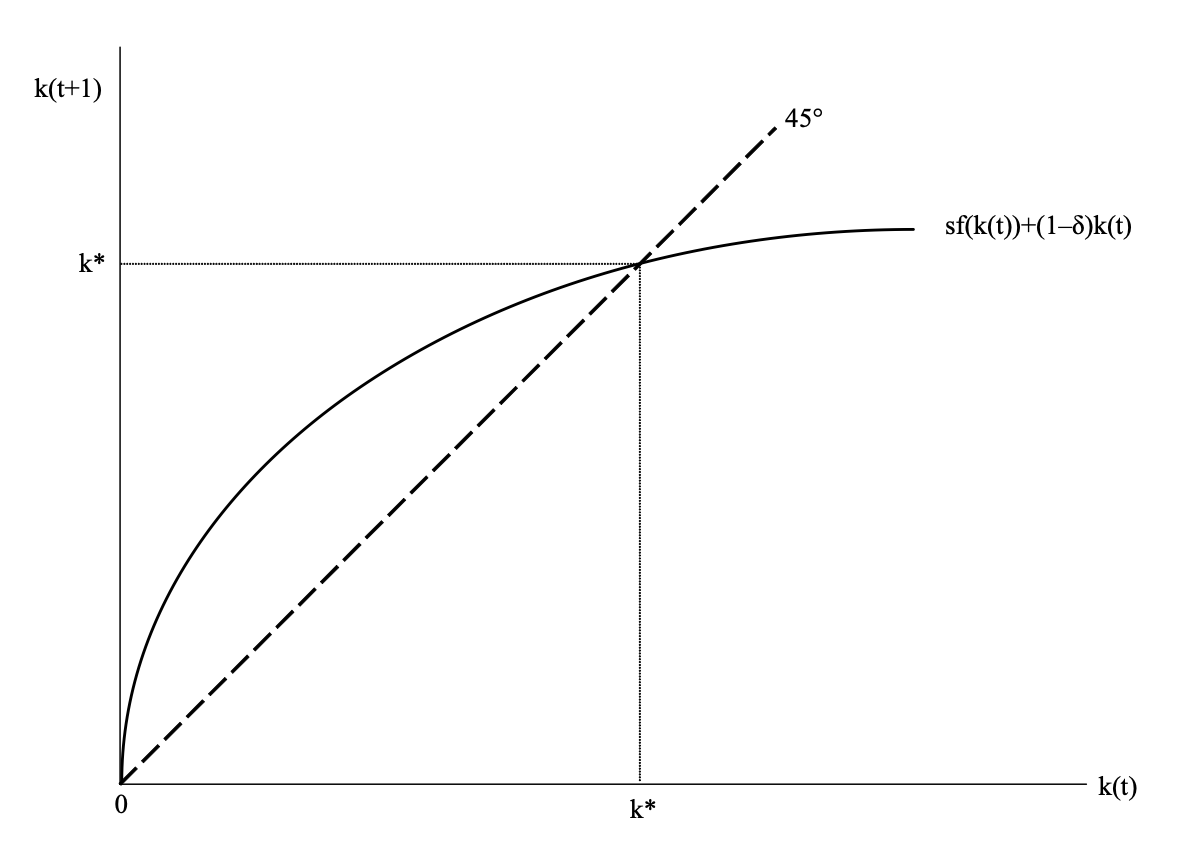
\includegraphics[width=0.85\linewidth]{images/solow_phase_diagram.png}
\end{center}
\noindent\textit{Reading the diagram.} This recovered diagram shows the special
case $n=g=0$, with $\delta>0$. The curved map is next period's capital; the
45-degree line is unchanged capital. Starting on the horizontal axis, move
vertically to the map, then horizontally to the 45-degree line to carry that
value into the next iteration. For $n>0$ or $g>0$, divide the map by $D$ as in
\eqref{eq:solow-discrete-map}.

A steady state is one particular equilibrium path. A transition from an
arbitrary initial stock is also an equilibrium path under the imposed saving
rule. Convergence does not make the transition cease to be an equilibrium.

\subsubsection{What grows on a balanced growth path?}

If $k_t=k^*$, then $y_t=f(k^*)$ and $c_t=(1-s)f(k^*)$ are constant. Yet
\begin{equation}\label{eq:solow-bgp}
\frac{Y_t}{L_t}=A_tf(k^*),\qquad
\frac{K_t}{L_t}=A_tk^*,\qquad
Y_t=A_tL_tf(k^*).
\end{equation}
Output and capital per worker grow at gross rate $1+g$; their aggregates grow
at $D$. With no technical progress, there is no sustained growth per worker on
this path, even if the population and total output keep growing.

For Cobb--Douglas, solve $s(k^*)^\alpha=d_Dk^*$:
\begin{equation}\label{eq:solow-cd-steady}
k^*=\left(\frac{s}{d_D}\right)^{1/(1-\alpha)},\qquad
y^*=\left(\frac{s}{d_D}\right)^{\alpha/(1-\alpha)}.
\end{equation}
A higher saving rate raises the long-run level of output per effective worker.
Holding the technology path fixed, it does not change the long-run growth rate
of output per worker. Its steady-state level elasticity is
\begin{equation}
\frac{\partial\log y^*}{\partial\log s}=\frac{\alpha}{1-\alpha}.
\end{equation}
This comparison holds other determinants fixed. It is not a causal estimate
from a cross-country correlation between saving and income.

\subsubsection{Saving, rebuilding, and conditional convergence}

Suppose an economy starts on its old balanced growth path and permanently
raises $s$. At the time of the change, $K$, $A$, and $L$ are inherited, so output
is unchanged and consumption falls. Higher investment raises future $K$; output
per worker then grows faster during the transition. As diminishing returns
reduce the extra investment generated by another unit of capital, $k$ approaches
its new, higher steady state. Long-run growth per worker returns to $g$.

This explains why an investment expansion can have a lasting level effect
without a lasting growth-rate effect. It does not establish that any observed
investment campaign will be productive: the one-good benchmark abstracts from
project selection, idle capacity, financing, and heterogeneous returns.

A one-time loss of physical capital, with technology, labor, and saving behavior
unchanged, lowers $k$. The high marginal product at the lower stock supports
rebuilding toward the same path. Actual disasters can also destroy skills,
institutions, and technology, so this experiment isolates a capital-loss
mechanism rather than predicting every recovery.

The convergence result is conditional on the determinants of $k^*$ and the
technology path. A low-income economy with a low saving rate or low productivity
need not grow faster than a richer economy already close to a higher path.
Income alone does not tell us distance from the relevant steady state.

\subsubsection{Local convergence speed}

Let $x_t=k_t-k^*$. A first-order Taylor expansion at $k^*$ gives
\begin{align}
k_{t+1}&=\Phi(k^*)+\Phi'(k^*)x_t+O(x_t^2),\\
x_{t+1}&\approx\phi x_t,\qquad
\phi\equiv\frac{1-\delta+sf'(k^*)}{D}.
\end{align}
Because $sf'(k^*)<sf(k^*)/k^*=d_D$, we have $0<\phi<1$. Iterating the
linearized system yields
\begin{equation}\label{eq:solow-discrete-speed}
x_t\approx\phi^t x_0,\qquad
\lambda_D=-\log\phi>0,\qquad
T_{1/2}\approx\frac{\log2}{\lambda_D}.
\end{equation}
$\phi$ is persistence; a larger $\phi$ means slower adjustment. $\lambda_D$ is
the corresponding decay rate per period, and $T_{1/2}$ is the local half-life
of a deviation. The original nonlinear path need not have this half-life far
from its steady state.

For Cobb--Douglas, $sf'(k^*)=\alpha d_D$, so
\begin{equation}
\phi=1-\frac{(1-\alpha)d_D}{D}.
\end{equation}
Adjustment is gradual because productive capacity is a stock. Investment can
change immediately, but only accumulated investment changes that stock.

\subsection{Solow model in continuous time}\label{solow-model-in-continuous-time}

\subsubsection{The same mechanism with continuous adjustment}

Now use continuous rates $\dot L/L=n$, $\dot A/A=g$, and depreciation rate
$\delta\geq0$, with $b\equiv n+g+\delta>0$. These are rates per unit of time;
they are not numerically identical to finite-period percentage changes. Write
\begin{equation}
\dot K=sF(K,AL)-\delta K,\qquad k=\frac{K}{AL},\qquad y=f(k).
\end{equation}
Log differentiation of the definition of $k$, followed by substitution, gives
\begin{align}
\frac{\dot k}{k}
&=\frac{\dot K}{K}-\frac{\dot A}{A}-\frac{\dot L}{L},\\
&=\frac{sY}{K}-\delta-g-n,\\
\dot k&=s\frac{Y}{AL}-(n+g+\delta)k
       =sf(k)-bk\equiv G(k).\label{eq:solow-continuous}
\end{align}
New investment increases capital intensity; depreciation, population growth,
and technical progress reduce it for a given aggregate stock. Technical
progress still raises productive possibilities: it reduces $k$ here because
each worker now represents more effective labor.

For a short time interval $\Delta t$, effective labor grows by approximately
$1+(n+g)\Delta t$ and depreciation is approximately $\delta\Delta t$. Applying
the discrete accounting over that interval gives
\begin{equation}
k(t+\Delta t)-k(t)
=\left[sf(k(t))-bk(t)\right]\Delta t+o(\Delta t).
\end{equation}
Divide by $\Delta t$ and take its limit to obtain
\eqref{eq:solow-continuous}. This explains why the continuous break-even rate
is $b$, whereas the exact discrete expression contains the product $ng$.

The positive steady state satisfies $sf(k^*)=bk^*$; $G(k)>0$ below it and
$G(k)<0$ above it. On the balanced growth path, $Y/L$ and $K/L$ grow at $g$,
$Y$ and $K$ grow at $n+g$, and $K/Y=s/b$. Under competitive pricing the net
instantaneous real return is $r=f'(k)-\delta$.

\subsubsection{Local approximation and an exact Cobb--Douglas solution}

Linearizing the law of motion around its steady state gives
\begin{align}
\dot k&\approx G'(k^*)(k-k^*),\\
G'(k^*)&=sf'(k^*)-b<0,\\
k(t)-k^*&\approx[k(0)-k^*]e^{-\lambda_Ct},
\qquad \lambda_C\equiv b-sf'(k^*)>0.\label{eq:solow-continuous-speed}
\end{align}
The exponential expression solves the \emph{linearized} system. It is generally
only a local approximation to the original nonlinear equation. For
Cobb--Douglas, $\lambda_C=(1-\alpha)b$ and the local half-life is
$\log2/[(1-\alpha)b]$.

Cobb--Douglas also permits an exact solution using a different variable. Set
$z(t)=k(t)^{1-\alpha}$ and differentiate:
\begin{align}
\dot z
&=(1-\alpha)k^{-\alpha}\dot k,\\
&=(1-\alpha)k^{-\alpha}(sk^\alpha-bk)
 =(1-\alpha)(s-bz).
\end{align}
This is a linear equation in $z$, with steady state $z^*=s/b$. Its solution
and the implied capital path are
\begin{align}
z(t)&=\frac{s}{b}+\left[z(0)-\frac{s}{b}\right]
 e^{-(1-\alpha)bt},\\
k(t)&=\left\{\frac{s}{b}+\left[k(0)^{1-\alpha}-\frac{s}{b}\right]
 e^{-(1-\alpha)bt}\right\}^{1/(1-\alpha)}.\label{eq:solow-exact-path}
\end{align}
Capital approaches its steady state without arriving there at a finite date
unless it starts there. ``Time to convergence'' must therefore specify a
tolerance or a half-life, rather than an exact date of arrival.

\subsection{The Golden Rule and the cost of saving}\label{golden-rate}

More saving raises steady-state output, but output is not consumption. To
maintain a larger capital stock, the economy must devote more resources to
investment. The Golden Rule asks which balanced growth path provides the
largest consumption per effective worker, holding the technology and labor
paths fixed.

In continuous time, a stationary $k$ requires investment $bk$, so feasible
steady-state consumption is
\begin{equation}\label{eq:solow-gr-consumption}
c^*=f(k)-bk.
\end{equation}
Maximize this expression over $k$:
\begin{align}
\frac{dc^*}{dk}&=f'(k)-b,\\
f'(k_{\mathrm{GR}})&=b=n+g+\delta,\qquad
\frac{d^2c^*}{dk^2}=f''(k)<0.\label{eq:solow-gr}
\end{align}
One extra unit of capital adds $f'(k)$ to output but requires $b$ units of
investment per unit of time to maintain its intensity. At the Golden Rule,
these marginal amounts are equal. Equivalently, the net marginal return
$f'(k_{\mathrm{GR}})-\delta$ equals $n+g$.

The saving rate that supports this stock satisfies
\begin{equation}
s_{\mathrm{GR}}=\frac{bk_{\mathrm{GR}}}{f(k_{\mathrm{GR}})}.
\end{equation}
For Cobb--Douglas, substitute
$\alpha k_{\mathrm{GR}}^{\alpha-1}=b$:
\begin{equation}
k_{\mathrm{GR}}=\left(\frac{\alpha}{b}\right)^{1/(1-\alpha)},
\qquad s_{\mathrm{GR}}=\alpha.
\end{equation}
In discrete time the argument is the same with $d_D$ replacing $b$:
$c^*=f(k)-d_Dk$ and $f'(k_{\mathrm{GR}})=d_D$. The Cobb--Douglas saving share
is again $\alpha$ under this timing convention.

\begin{blueblock}
\textbf{A welfare boundary.}
The Golden Rule maximizes consumption \emph{across balanced growth paths}.
Solow has not specified a utility function, discounting, or how to value the
consumption losses during a transition. It therefore does not establish that
moving toward the Golden Rule maximizes intertemporal welfare.
\end{blueblock}

If the initial steady state lies below $k_{\mathrm{GR}}$, raising saving toward
$s_{\mathrm{GR}}$ increases eventual consumption but requires sacrificing
consumption while capital is built. If it lies above $k_{\mathrm{GR}}$, reducing
saving toward the Golden Rule can raise both current and eventual consumption.
Investment is then maintaining more capital than is useful for maximizing
steady-state consumption. A high investment share alone is therefore not a
welfare criterion. Ramsey will specify preferences and make the transition
trade-off part of the saving decision; OLG will examine dynamic efficiency in
an economy with different generations.

\subsection{Extensions}

Solow model with money
\begin{itemize}
  \item Purvis, Douglas D. “Introducing Useful Money into a Growth Model.” The Canadian Journal of Economics / Revue Canadienne d’Economique 4, no. 3 (1971)
\end{itemize}

Augmented Solow model

\begin{itemize}
  \item N. Gregory Mankiw, David Romer, David N. Weil, A Contribution to the Empirics of Economic Growth, The Quarterly Journal of Economics, Volume 107, Issue 2, May 1992, Pages 407–437
\end{itemize}

AK model (often treated as a tool to introduce endogeneous growth model)

\begin{itemize}
  \item Romer, Paul M. (1986). "Increasing Returns and Long-Run Growth". Journal of Political Economy. 94 (5): 1002–1037.
\end{itemize}

Malthus to Solow (unified growth theory)

\begin{itemize}
  \item Hansen, Gary, D., and Edward C. Prescott. 2002. "Malthus to Solow ." American Economic Review, 92 (4): 1205–1217.
\end{itemize}

% !TEX root = ../macro.tex
\section{Ramsey Model}\label{sec:ramsey}

Solow determines accumulation from a given saving share. Ramsey asks how much
to consume and save when households value consumption at different dates.
The change adds a choice, a price for postponing consumption, and a boundary
condition that selects an admissible path.

\subsection{From a saving rule to a saving decision}

Suppose two economies have the same current income. In one, income is expected
to rise; in the other, a disruption has temporarily reduced production. A rule
$S=sY$ makes saving move proportionally with current output in both cases.
It cannot tell us whether households want to smooth a temporary loss, prepare
for lower future income, or invest in a newly productive opportunity.

One response would be to make $s$ a function of income or the interest rate.
But then we would still need to explain that function and how it changes when
expectations or policy change. Instead, specify what consumption is worth,
what saving buys, and which paths the household can finance. A saving rate
will emerge from those choices rather than being the starting rule.

Start with the experiment of consuming one unit less today. Saving that unit
provides a return tomorrow. The household compares the utility lost now with
the discounted utility of that future consumption. This suggests an optimality
condition across adjacent dates. It cannot yet determine the level of
consumption: a household with little wealth cannot finance every path with
the right slope. We will need feasibility and a terminal restriction as well.

The planner and household formulations then answer related questions. The
planner allocates real resources; a household takes wages and returns as given.
Their allocations coincide in the competitive benchmark under the conditions
stated below. Taxes can separate the private return from the social product,
which is why decentralization matters for the final section.

Ramsey's original contribution was a saving problem; the presentation here is
the modern discounted Ramsey--Cass--Koopmans benchmark, rather than a literal
reproduction of the 1928 objective.\footnote{Frank P. Ramsey (1928), ``A
Mathematical Theory of Saving,'' \textit{Economic Journal}, 38(152), 543--559.
\url{https://doi.org/10.2307/2224098}.}

% BEGIN ORIGINAL COURSE ASSUMPTIONS - retained, not typeset
% \subsection{Assumptions}\label{assumptions}
% 
% 
% 
% \begin{itemize}
%   \item Same as Solow Model
%     \begin{itemize}
%     \tightlist
%       \item Production Function in the Harrold neutrality form
%       \item \textbf{Exogenous Variables:}
%       \item Population growth rate$=n$
%       \item Technology growth rate$=g$
%       \item Depreciation rate$=0$ (for simplicity)
%       \item And most of all, the technological growth rate is assumed as $a$.
%     \end{itemize}
%   \item Firm
%     \begin{itemize}
%     \tightlist
%       \item Perfect competitive firms, or homogenous firms, or representive firms
%       \item Hire workers and capital in competitive factor markets
%       \item Each has the production function $Y=F(K,AL)$
%       \item Firms are owned by the families, meaning the revenue goes straight to
%       latter
%     \end{itemize}
%   \item Household
%     \begin{itemize}
%     \tightlist
%       \item Homogenous families.
%       \item Population growth of each household is assumed as $n$.
%       \item Each member in a household provides one unit of labor.
%       \item Income of a household is the sum of the labor revenue subsum, the capital revenue subsum and the firm revenue share subsum.
%       \item A household should and must maximize the utility.
%       \item Degree of patience denoted as discount factor $\beta=\frac{1}{1+\rho}$, and $\rho$ is the discount rate.
%     \end{itemize}
% \end{itemize}
% 
% 
% 
% \begin{blueblock}
% \begin{note}[Rule of Prohibiting Ponzi Schemes]
% Conconstraint in Ramsey model is also called Prohibiting Ponzi Schemes Rule. It forbids the household to do a scam of rolling over debt by repeatedly borrowing. Yet in real life, many people are doing this as a harmless way to ralex debt pressure.
% \end{note}
% \end{blueblock}
% 
% END ORIGINAL COURSE ASSUMPTIONS

\Needspace{34\baselineskip}
\subsection{Assumptions}\label{assumptions}

The economic environment follows Solow. The new ingredient is a household
objective, so the map separates its choices from technology and market clearing.

\begin{modelsetup}
\begin{modelcondition}{01}{Technology and resources}
A closed, one-good economy without government in the baseline:
\[
Y=F(K,AL),\quad Y=C+I.
\]
Production has the Solow properties.
\end{modelcondition}
\begin{modelcondition}{02}{Given states and paths}
Positive initial stocks. Labor and technology grow exogenously:
\[
\dot L/L=n,\qquad \dot A/A=g.
\]
The course benchmark sets $\delta=0$.
\end{modelcondition}
\begin{modelcondition}{03}{Households}
Identical, price-taking dynasties own capital. Each member supplies one unit
of labor and chooses consumption over time.
\end{modelcondition}
\begin{modelcondition}{04}{Preferences}
Utility is defined over consumption per person, $x=C/L$:
\[
\int_0^\infty e^{-\rho t}L(t)u(x(t))\,dt.
\]
Patience and curvature affect saving.
\end{modelcondition}
\begin{modelcondition}{05}{Firms and prices}
Competitive firms maximize profits. Rental income and wages go to households;
profits are zero under constant returns.
\end{modelcondition}
\begin{modelcondition}{06}{Feasible optimal paths}
Capital is inherited; consumption is chosen. Feasibility, optimality, market
clearing, and terminal conditions jointly select a path.
\end{modelcondition}
\end{modelsetup}

\subsubsection{Notation and the course simplifications}

Use $K,C,Y$ for aggregates and $x=C/L$ for consumption per person. Reserve
$k=K/(AL)$ and $c=C/(AL)$ for quantities per effective worker, so $x=Ac$.
Technology growth is denoted by $g$ throughout. We retain the course's
zero-depreciation benchmark; $\delta$ remains visible in the formulas so that
setting $\delta=0$ is explicit. Full depreciation, $\delta=1$, will be used
only in a separately labeled discrete-time example.

Preferences have marginal utility $u'(x)=x^{-\theta}$, $\theta>0$:
\begin{equation}\label{eq:ramsey-utility}
u(x)=\begin{cases}
 x^{1-\theta}/(1-\theta),&\theta\ne1,\\
 \log x,&\theta=1.
\end{cases}
\end{equation}
In this deterministic model, $1/\theta$ measures willingness to substitute
consumption across time. Higher $\rho$ reduces the weight on future utility.
Assume $\rho>n\geq0$, $g\geq0$, and
\begin{equation}\label{eq:ramsey-effective-discount}
\eta\equiv\rho-n-(1-\theta)g>0.
\end{equation}
These are sufficient restrictions for finite utility on the balanced growth
path used below. Weighting by $L(t)$ means the dynasty values the utility of
all its members; choosing a different population welfare criterion would change
the normalization. The original lists are retained in comments immediately
above this section for comparison.

\subsubsection{No-Ponzi restrictions and transversality}

A household's total wealth $B$ satisfies
\begin{equation}
\dot B=rB+wL-C,
\end{equation}
where $r$ is the net real return and $w$ the wage per person. A no-Ponzi
restriction requires
\begin{equation}\label{eq:ramsey-npg}
\liminf_{T\to\infty}e^{-\int_0^T r(v)\,dv}B(T)\geq0.
\end{equation}
Borrowing must ultimately be supported by resources rather than by a negative
terminal present value of wealth. Refinancing a loan is not, by itself, a
Ponzi scheme: future income can support repayment.

A transversality condition instead concerns optimality. In the planner's
normalized problem below it takes the standard form
\begin{equation}\label{eq:ramsey-tvc}
\lim_{t\to\infty}e^{-\eta t}u'(c(t))k(t)=0.
\end{equation}
It rules out leaving resources with positive limiting discounted utility value
when consuming more would improve the allocation. It does not require the
capital stock itself to approach zero. Feasibility and an Euler equation alone
need not select the optimal infinite-horizon path.

\subsection{Solving the consumption--saving problem}

\subsubsection{The planner's problem and decentralization}\label{central-planners-problem}

For continuous time, the planner chooses consumption with inherited $K(0)$:
\begin{equation}\label{eq:ramsey-planner}
\begin{split}
\max_{\{C(t)\}}\;&\int_0^\infty e^{-\rho t}L(t)u(C(t)/L(t))\,dt,\\
\text{s.t. }&\dot K=F(K,AL)-\delta K-C,\qquad K\geq0,\ C>0.
\end{split}
\end{equation}
Consumption uses current output; the residual, net of depreciation, changes
the capital stock. In a decentralized economy, a household uses its budget
constraint instead. Competitive factor pricing gives
\begin{equation}\label{eq:ramsey-factor-prices}
q=f'(k),\qquad r=q-\delta,\qquad
w=A\left[f(k)-kf'(k)\right].
\end{equation}
$q$ is the rental payment before depreciation. The net return $r=q-\delta$
and a discrete-time gross return $R=1+q-\delta=1+r$ are different objects.

With constant returns, factor incomes exhaust output. Firms' dividends are
not an additional source of aggregate goods on top of $Y$. In equilibrium,
aggregate household wealth equals capital, $B=K$, so the household budgets
consolidate into \eqref{eq:ramsey-planner}'s resource constraint. With identical
preferences, competitive prices, and no taxes, externalities, or financing
frictions, the planner allocation can be supported as a competitive allocation.
This equivalence must be checked again when the environment changes.

\subsubsection{Lagrangian: the adjacent-date trade-off}\label{method-of-lagrangian}

First isolate discrete time with $A=L=1$ and $n=g=0$. This makes timing visible
without carrying growing denominators; it is a restricted version of the model.
The planner solves
\begin{equation}
\max_{\{c_t,k_{t+1}\}}\sum_{t=0}^\infty\beta^tu(c_t),\qquad
c_t+k_{t+1}=f(k_t)+(1-\delta)k_t,
\end{equation}
where $k_0$ is given, $0<\beta<1$, and $0\leq\delta\leq1$. Writing
$\beta=1/(1+\rho)$ defines a discrete-time rate of time preference; the
continuous-time convention uses $e^{-\rho t}$.

Use current-utility multipliers $\lambda_t$:
\begin{equation}
\mathscr L=\sum_{t=0}^\infty\beta^t
\left\{u(c_t)+\lambda_t[f(k_t)+(1-\delta)k_t-c_t-k_{t+1}]\right\}.
\end{equation}
At an interior solution, differentiate with respect to $c_t$ and $k_{t+1}$:
\begin{align}
\lambda_t&=u'(c_t),\\
\lambda_t&=\beta\lambda_{t+1}[f'(k_{t+1})+1-\delta].
\end{align}
Substitution gives the Euler equation
\begin{equation}\label{eq:ramsey-discrete-euler}
u'(c_t)=\beta R_{t+1}u'(c_{t+1}),\qquad
R_{t+1}=f'(k_{t+1})+1-\delta.
\end{equation}
One unit saved at $t$ earns its return at $t+1$, when the new capital is used.
The utility cost today equals the discounted marginal gain tomorrow. For CRRA,
\begin{equation}
\frac{c_{t+1}}{c_t}=(\beta R_{t+1})^{1/\theta}.
\end{equation}
This determines consumption growth given the return, not the entire consumption
path. With no bequest motive and the usual concavity conditions, the terminal
condition is $\lim_{t\to\infty}\beta^tu'(c_t)k_{t+1}=0$. In a finite-horizon
exercise a terminal stock may be set to zero; that is not the same as imposing
$k_t\to0$ in this infinite-horizon economy.

\subsubsection{Hamiltonian: saving with continuous adjustment}\label{method-of-hamiltonian-equation-optimal-control}

Return to continuous time with population and technology growth. From
$k=K/(AL)$ and $c=C/(AL)$,
\begin{equation}\label{eq:ramsey-capital-motion}
\dot k=f(k)-c-bk,\qquad b\equiv n+g+\delta.
\end{equation}
For $\theta\ne1$, substitute $x=Ac$ and $L=L_0e^{nt}$ into utility:
\begin{equation}
e^{-\rho t}Lu(Ac)
=L_0A_0^{1-\theta}e^{-\eta t}\frac{c^{1-\theta}}{1-\theta}.
\end{equation}
The positive constant in front does not change choices. For log utility,
$\log(Ac)=\log A+\log c$; the $\log A$ term is independent of the allocation.
The normalized problem therefore discounts $u(c)$ at $\eta$ in either case.

Its current-value Hamiltonian is
\begin{equation}
\mathcal H=u(c)+\mu[f(k)-c-bk].
\end{equation}
The control condition and current-value costate equation are
\begin{align}
\mathcal H_c=0&\quad\Longrightarrow\quad \mu=u'(c),\\
\dot\mu=\eta\mu-\mathcal H_k
&=\left[\eta+b-f'(k)\right]\mu.
\end{align}
$\mu$ is the current utility value of an additional unit of normalized capital.
The factor $\eta$ belongs in the current-value costate equation; a
present-value costate would instead absorb the discount factor. These are two
representations of the same problem, not an assertion that patience is irrelevant.

Differentiate $\mu=c^{-\theta}$ and use
$\eta+b=\rho+\delta+\theta g$:
\begin{align}
\frac{\dot\mu}{\mu}&=-\theta\frac{\dot c}{c}
 =\eta+b-f'(k),\\
\frac{\dot c}{c}
&=\frac{f'(k)-\delta-\rho-\theta g}{\theta}.
\label{eq:ramsey-normalized-euler}
\end{align}
Consumption per person is $x=Ac$, so
\begin{equation}\label{eq:ramsey-person-euler}
\frac{\dot x}{x}=g+\frac{\dot c}{c}
 =\frac{r-\rho}{\theta}.
\end{equation}
A high return makes future consumption relatively attractive; impatience favors
consumption now. Curvature determines how strongly consumption growth responds.
Population growth affects resources and welfare weights, but cancels from this
per-person Euler equation under the dynasty objective specified above.

Setting $\delta=0$ recovers the course benchmark. Setting $g=n=0$ also removes
the growth normalization. At $\rho=0$ the intertemporal trade-off changes, and
an infinite-horizon undiscounted problem needs its own welfare criterion; it is
not obtained simply by deleting discounting from every infinite integral.

\subsubsection{Bellman and HJB: valuing the remaining opportunities}\label{method-of-bellman-equation-dynamic-programming}

For the stationary discrete-time version, let $V(k)$ be the value of starting
with capital $k$. Choose next period's capital $k'$:
\begin{equation}
V(k)=\max_{k'}\left\{u(f(k)+(1-\delta)k-k')+\beta V(k')\right\},
\end{equation}
with feasible $k'\geq0$ and positive current consumption. At an interior optimum,
\begin{align}
u'(c)&=\beta V'(k'),\\
V'(k)&=u'(c)[f'(k)+1-\delta].
\end{align}
The second line is the envelope condition: the effect of the optimal choice's
response drops out at the optimum. Apply it at $k'$ in the first line to recover
\eqref{eq:ramsey-discrete-euler}. The Lagrangian and Bellman methods are pricing
the same marginal transfer of resources between dates.

\textbf{A case with an exact saving rule.}
Take $u(c)=\log c$, $f(k)=k^\alpha$, and full depreciation $\delta=1$ only for
this example. Guess $V(k)=a+d\log k$. The first-order condition gives
\begin{equation}
\frac{1}{k^\alpha-k'}=\frac{\beta d}{k'},\qquad
\frac{k'}{k^\alpha}=\frac{\beta d}{1+\beta d}.
\end{equation}
Matching the coefficient of $\log k$ in the Bellman equation yields
$d=\alpha(1+\beta d)$, hence
\begin{equation}\label{eq:ramsey-exact-saving}
d=\frac{\alpha}{1-\alpha\beta},\qquad
k'=\alpha\beta k^\alpha,\qquad c=(1-\alpha\beta)k^\alpha.
\end{equation}
A constant saving share can emerge from optimization in this special case. Its
value depends on preferences and technology; the result does not make a
constant saving share general once depreciation or utility changes.

In normalized continuous time, dynamic programming gives the HJB equation
\begin{equation}
\eta V(k)=\max_c\{u(c)+V'(k)[f(k)-c-bk]\}.
\end{equation}
The control condition is $u'(c)=V'(k)$. Differentiate using the envelope theorem:
\begin{equation}
\eta V'(k)=V''(k)\dot k+V'(k)[f'(k)-b].
\end{equation}
Along the path, $\dot\mu=V''(k)\dot k$ with $\mu=V'(k)$, giving the same
costate equation and consumption Euler equation as the Hamiltonian. The value
function summarizes all future opportunities; the terminal and feasibility
conditions remain part of the underlying problem.

\subsection{Intertemporal equilibrium and economic adjustment}

\subsubsection{Steady state and the two loci}

The continuous-time equilibrium combines
\begin{equation}\label{eq:ramsey-system}
\begin{split}
\dot k&=f(k)-c-bk,\\
\dot c&=\frac{c}{\theta}[f'(k)-\delta-\rho-\theta g],
\end{split}
\end{equation}
with given $k(0)$ and \eqref{eq:ramsey-tvc}. A positive normalized steady state
satisfies
\begin{equation}\label{eq:ramsey-steady}
f'(k^*)=\delta+\rho+\theta g,\qquad c^*=f(k^*)-bk^*.
\end{equation}
The production assumptions give a unique positive $k^*$. Strict concavity gives
$f(k^*)/k^*>f'(k^*)>b$, where the second inequality is $\eta>0$, so $c^*>0$.
On this balanced growth path, consumption per person grows at $g$, aggregate
consumption at $n+g$, and the net return is $r^*=\rho+\theta g$.

For $c>0$, the $\dot c=0$ locus is vertical at $k^*$. Consumption grows to its
left and falls to its right. The $\dot k=0$ locus is $c=f(k)-bk$; capital grows
below it and falls above it. If $b>0$, its maximum is the Golden Rule stock,
where $f'(k_{\mathrm{GR}})=b$. Neither locus, by itself, is an equilibrium path.

\begin{center}
\begin{minipage}{\linewidth}
\centering
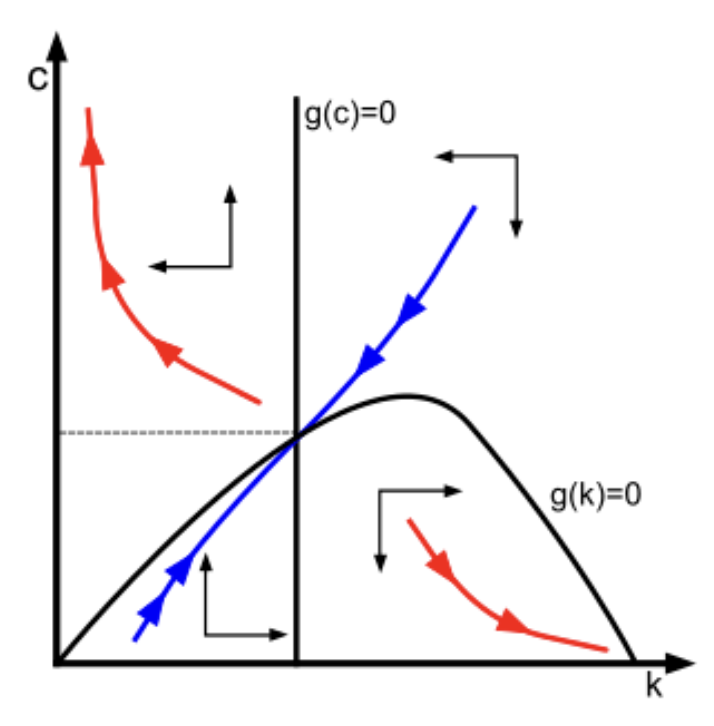
\includegraphics[width=0.48\linewidth]{images/ramsey_phase_diagram.png}
\par\medskip\RaggedRight
\noindent\textit{Reading the diagram.} The vertical line is $\dot c=0$; the
curved resource locus is $\dot k=0$. The blue curve depicts the stable path,
with arrows toward their intersection. The red paths illustrate departures
that do not satisfy the required long-run conditions. The sketch assumes a
hump-shaped resource locus and $k^*<k_{\mathrm{GR}}$.
\end{minipage}
\end{center}

\subsubsection{Why consumption can jump while capital cannot}

Capital is a state inherited from previous investment. Consumption is a control:
a household can change spending immediately, but cannot instantly create a
new stock of machines. For a given $k(0)$, different initial consumption choices
produce different candidate paths under \eqref{eq:ramsey-system}. Most fail
feasibility or the terminal condition. The saddle path selects initial
consumption as well as the later transition; it does not require every variable
to start at its steady state.

A one-time destruction of physical capital, with all other fundamentals
unchanged, moves the state leftward. Consumption adjusts onto the stable path.
The low stock supports a high return and rebuilding, while the loss of resources
constrains current spending. Actual disasters may also damage skills or
technology, which would change the destination rather than just the initial state.

A credible announcement about future productivity or taxation can change
consumption before it changes current output: the household evaluates future
income and returns when choosing today's spending. This model isolates that
intertemporal mechanism. It omits borrowing constraints, income risk, and
different marginal propensities to consume, so its representative consumption
response is not an empirical claim about every household.

\subsection{Linearization and the saddle path}

\subsubsection{The local system and its eigenvalues}

Let $\Delta k=k-k^*$ and $\Delta c=c-c^*$. In the order $(k,c)$, the first-order
system is
\begin{equation}\label{eq:ramsey-jacobian}
\begin{pmatrix}\dot{\Delta k}\\\dot{\Delta c}\end{pmatrix}
\approx
J\begin{pmatrix}\Delta k\\\Delta c\end{pmatrix},\qquad
J=\begin{pmatrix}\eta&-1\\ z&0\end{pmatrix},\quad
z\equiv\frac{c^*f''(k^*)}{\theta}<0.
\end{equation}
The top-left entry is $f'(k^*)-b=\eta$; the bottom-right entry vanishes because
the consumption growth bracket is zero at the steady state. Thus
\begin{equation}
\det(\lambda I-J)=\lambda^2-\eta\lambda+z=0,\qquad
\lambda_{\pm}=\frac{\eta\pm\sqrt{\eta^2-4z}}{2}.
\end{equation}
Since $z<0$, $\lambda_-<0<\lambda_+$. The local system has one stable and one
unstable direction. This is the mathematical reason a boundary condition is
needed to select consumption for the inherited capital stock.

For a stable eigenvector $(1,m)$, the first row implies
$m=\eta-\lambda_->0$. The local stable path is therefore
\begin{align}
\Delta c(0)&\approx m\Delta k(0),\\
\Delta k(t)&\approx\Delta k(0)e^{\lambda_-t},\\
\Delta c(t)&\approx m\Delta k(0)e^{\lambda_-t}.
\end{align}
The positive convergence speed is $-\lambda_-$; its local half-life is
$\log2/(-\lambda_-)$. The exponential solution is exact for the linearized
system, and generally approximate for the original nonlinear transition.

\subsubsection{The same restriction by undetermined coefficients}

Alternatively, conjecture a local policy $\Delta c=m\Delta k$. From the first
linearized equation, $\dot{\Delta k}=(\eta-m)\Delta k$. Differentiating the
conjecture and using the second equation gives
\begin{equation}
m(\eta-m)\Delta k=z\Delta k,\qquad m^2-\eta m+z=0.
\end{equation}
Choose the positive root $m=\lambda_+$, so $\eta-m=\lambda_-<0$. This recovers
the same stable policy. Choosing the decaying direction is not a free change
to initial capital; it is the restriction on the consumption choice implied
by admissibility and optimality.

\subsection{Maximizing welfare}\label{maximizing-welfare}

Similiar to the concept of golden rate in Solow model, Ramsey model also provide a glimpse of maximized consumption.

At the steady state
\begin{align}
&c^{*}= F(k^{*})-\delta k^{*}
\\&\Rightarrow k^*_{gold}=\underset{k^*}{\text{argmax}} \;c^{*}
\end{align}











\subsection[Taxation and capital accumulation (planned)]{Taxation and capital accumulation}
\textit{Planned section.} Compare lump-sum and distortionary taxes in the neoclassical growth framework.
Separate effects on steady-state capital from effects along the transition.

% !TEX root = ../macro.tex
\section{OLG Model}\label{sec:olg}

Ramsey assigns intertemporal choices to a dynasty that continues indefinitely.
Now separate a person's lifetime from the economy's lifetime. People work,
retire, and leave; new people arrive. Saving remains an optimal choice, but
the ownership of assets and the identity of the people paying for transfers
must be tracked by generation.

\subsection{From retirement needs to overlapping generations}

\subsubsection{An economy continues after its current savers have died}

Imagine looking at households' balance sheets at one date. Some people are
building retirement assets from wages; others are spending assets accumulated
earlier. A single consumption total conceals these opposite positions. A policy
that taxes workers and pays retirees changes the resources of different people,
even when it leaves aggregate resources unchanged at the moment of payment.

One response would be to add age labels to the Ramsey household. But if an
altruistic dynasty still pools all resources and values every descendant,
those labels need not change the underlying allocation problem. To isolate
generational turnover, instead let each person value only consumption within
his or her own finite life. Give the young labor income and the old a need to
finance consumption without working. Then ask what assets can carry resources
between these stages, and who supplies the counterpart to those claims.

Two periods are the smallest useful life cycle: one for work and saving, one
for retirement and spending. New workers arrive while earlier workers retire.
The approximation does not describe every age or predict a literal retirement
age. It makes the relation between life-cycle saving, asset ownership, and
population replacement visible with only two age groups.

\subsubsection{Choose a way to finance retirement, then close the economy}

Start with physical capital as the only asset. A young person acquires capital
claims; next period those claims pay rental income and the value of surviving
capital. Retirees consume the proceeds. A wage and a return determine an
individual saving choice, but they are not arbitrary economy-wide inputs:
workers' saving determines the next capital stock, which determines the return
those same workers receive when old. This closes the market model.

An alternative is a transfer from next period's workers. That alternative
cannot simply be assumed to be a private enforceable contract with people who
have not yet been born. A pension system or a government issuing debt adds an
institution capable of continuing across generations. We first solve the
capital-only economy, then introduce those institutions explicitly.

The production economy follows Diamond's OLG framework; the sequence of
questions above is a teaching reconstruction, not a claim about the author's
private thoughts.\footnote{Peter A. Diamond (1965), ``National Debt in a
Neoclassical Growth Model,'' \textit{American Economic Review}, 55(5),
1126--1150. Diamond's original model uses no depreciation; we keep general
$\delta$ and identify the full-depreciation course example separately.
\url{https://www.aeaweb.org/aer/top20/55.5.1126-1150.pdf}.}

\begin{blueblock}
\textbf{Meeting only once does not rule out intertemporal trade.}
A young person can save in capital and consume its payoff when old. That is
already an intertemporal allocation. The important limitation is that currently
living people cannot make ordinary private contracts with unborn generations.
Without bequests or altruistic links, no household represents the interests
of the infinite sequence of future entrants. Finite individual lives and an
infinite economic horizon can therefore have different welfare implications
from a single infinite-lived dynasty.
\end{blueblock}

% BEGIN ORIGINAL OLG COURSE ASSUMPTIONS - retained, not typeset
% \subsection{Assumptions}
% \begin{align}
% &C_{t}= L_{t} C_{1t}^{\text{young}}+L_{t-1}C_{2t}^{\text{old}} \text{ (where subscript 1 and 2 stands for age)}
% \\&L_{t}=(1+n)L_{t-1} \Rightarrow L_{t}=(1+n)^{t}L_{0}
% \\&S_{t}=s_{t}L(t)
% \end{align}
% END ORIGINAL OLG COURSE ASSUMPTIONS

\Needspace{12\baselineskip}
\subsection{Assumptions and the cohort timeline}\label{sec:olg-assumptions}

The cards state the full environment before solving it. Within a cohort people
are identical; across ages, their income, remaining lifetime, and asset position
differ. There is no single representative person for both age groups.

\begin{modelsetup}[1]
\begin{modelcondition}{01}{Dates, cohorts, and population}
Time is discrete, $t=0,1,\ldots$. A cohort of $L_t$ people is born at each date,
lives for two periods with certainty, and dies after its second period.
At date $t$, $L_t$ young coexist with $L_{t-1}$ old:
\[
L_t=NL_{t-1},\qquad N\equiv1+n>0,\qquad L_t=N^tL_0.
\]
The baseline takes $n\geq0$; the population comparison later also permits
$-1<n<0$ when the other conditions remain feasible. Each young person supplies
one unit of labor inelastically; the old supply none. Labor is $L_t$, whereas
total population is $L_t+L_{t-1}$. A model period is a life stage, not
necessarily a calendar year.
\end{modelcondition}
\begin{modelcondition}{02}{Goods, capital, and technology growth}
A closed economy produces one good, usable for consumption and capital.
There is no government, foreign trade, money, or public debt in the baseline.
Technology is fixed and normalized to one: $Y_t=F(K_t,L_t)$.
This is an explicit zero-technology-growth benchmark, so $k_t=K_t/L_t$ is
capital per worker, not per effective worker. Capital depreciates at
$0\leq\delta\leq1$ and surviving capital can be sold or consumed:
\[
Y_t+(1-\delta)K_t=C_t+K_{t+1}.
\]
General formulas retain $\delta$. The numerical and explicit full-depreciation
examples set $\delta=1$; that restriction is not needed for the general model.
\end{modelcondition}
\begin{modelcondition}{03}{Production restrictions}
Firms share a freely available technology. $F$ is continuous, twice
differentiable for positive inputs, positive there, with positive diminishing
marginal products and constant returns:
\[
F(\lambda K,\lambda L)=\lambda F(K,L),\qquad
f(k)\equiv F(k,1),\qquad Y_t/L_t=f(k_t).
\]
For $k>0$, assume
\[
\begin{gathered}
f(0)=0,\qquad f'(k)>0,\qquad f''(k)<0,\\
\lim_{k\downarrow0}f'(k)=\infty,\qquad
\lim_{k\to\infty}f'(k)=0.
\end{gathered}
\]
Cobb--Douglas, $f(k)=k^\alpha$ with $0<\alpha<1$, is a specified example,
not the only technology consistent with these conditions.
\end{modelcondition}
\begin{modelcondition}{04}{Households, ownership, and initial conditions}
There are many identical, price-taking people in each cohort. They receive
wages when young and asset income when old; firms belong to households and
any profits would accrue to their owners. No one values descendants' utility,
leaves a bequest, or receives an inheritance. The initially old are the
exception to the no-inherited-wealth statement: they enter date zero already
owning the given $K_0>0$, equally within their cohort. The young start with
labor income and no assets. Initially old consumption must be counted even
though their earlier saving decision lies outside the model's initial date.
\end{modelcondition}
\begin{modelcondition}{05}{Preferences, information, and choices}
A person born at $t$ chooses saving $a_t$ and consumption at ages one and two:
\[
U_t=u(c_{1,t})+\beta u(c_{2,t+1}),\qquad 0<\beta<1,
\]
\[
u(c)=\begin{cases}(c^{1-\theta}-1)/(1-\theta),&\theta>0,\ \theta\ne1,\\
\log c,&\theta=1.
\end{cases}
\]
There is no aggregate or individual uncertainty; the next return is correctly
anticipated. People take wages and returns as given, despite their joint
effect on equilibrium prices. There is no labor choice or liquidity shock.
Consumption is positive. The baseline interior optimum has $0<a_t<w_t$;
no borrowing or short sales of physical capital are allowed. Later pension
formulas must be checked against this asset constraint.
\end{modelcondition}
\begin{modelcondition}{06}{Firms, factor prices, and returns}
Competitive firms rent capital and hire labor at each date:
\[
\max_{K,L}\;F(K,L)-q_tK-w_tL.
\]
Interior demands imply $q_t=f'(k_t)$ and $w_t=f(k_t)-k_tf'(k_t)$.
Economic profits are zero under constant returns. The owner of a unit of
capital receives the rental payment and its remaining capital value:
\[
R_t=1-\delta+q_t,\qquad r_t=R_t-1=q_t-\delta.
\]
$R_t$ is a gross payoff, $r_t$ a net return, and $q_t$ a rental price.
Only with $\delta=1$ does $R_t=f'(k_t)$.
\end{modelcondition}
\begin{modelcondition}{07}{Budgets and age-specific consumption}
A person born at $t$ obeys
\[
c_{1,t}+a_t=w_t,\qquad c_{2,t+1}=R_{t+1}a_t.
\]
The old consume all their wealth and leave no assets after death. At date $t$,
$c_{2,t}$ is the consumption of cohort $t-1$, not the future consumption of
cohort $t$. Aggregate consumption and young people's asset purchases are
\[
C_t=L_tc_{1,t}+L_{t-1}c_{2,t},\qquad
\mathcal A_t=L_ta_t.
\]
We use $a_t$ for saving per young person to distinguish it from Solow's saving
share $s$. $\mathcal A_t$ corresponds to the original course notation for
aggregate young saving; it is not automatically national saving.
\end{modelcondition}
\begin{modelcondition}{08}{Market clearing and the equilibrium path}
Capital and labor demands equal their supplied stocks, $K_t^d=K_t$ and
$L_t^d=L_t$. Capital is the only asset, so young people's wealth at the end of
$t$ must equal next period's capital:
\[
K_{t+1}=\mathcal A_t=L_ta_t,\qquad Nk_{t+1}=a_t.
\]
Goods clearing must also hold:
\[
c_{1,t}+\frac{c_{2,t}}{N}+Nk_{t+1}
=f(k_t)+(1-\delta)k_t.
\]
An equilibrium is a path of allocations and prices satisfying household and
firm optimality, correct return expectations, and these clearing conditions,
starting from the specified initial ownership. No infinite-lived household's
transversality condition is imposed on the economy as a whole.
\end{modelcondition}
\end{modelsetup}

\subsubsection{Read a cohort's lifetime across dates}

\begin{center}
\begin{tabular}{lccc}
\hline
Cohort & Date $t-1$ & Date $t$ & Date $t+1$\\
\hline
Born at $t-1$ & Young, saves & Old, consumes & No longer alive\\
Born at $t$ & Not yet born & Young, saves & Old, consumes\\
Born at $t+1$ & Not yet born & Not yet born & Young, saves\\
\hline
\end{tabular}
\end{center}

Reading across a row gives one person's lifetime budget. Reading down a
column gives the economy's resources at one date. This distinction explains
why $c_{1,t}+c_{2,t+1}/R_{t+1}=w_t$ is an individual present-value budget,
whereas $c_{1,t}+c_{2,t}/N$ is current aggregate consumption per worker.
The two formulas combine different people and different dates.

\subsection{Household optimization and life-cycle saving}

\subsubsection{Budgets, multipliers, and the Euler condition}

Take $w_t>0$ and $R_{t+1}>0$ as given. Monotonic utility makes the two budgets
bind. With multipliers on resources remaining, write
\begin{equation}
\begin{split}
\mathscr L={}&u(c_{1,t})+\beta u(c_{2,t+1})\\
&+\lambda_{1,t}(w_t-c_{1,t}-a_t)
+\lambda_{2,t+1}(R_{t+1}a_t-c_{2,t+1}).
\end{split}
\end{equation}
At an interior optimum,
\begin{align}
u'(c_{1,t})&=\lambda_{1,t},\\
\beta u'(c_{2,t+1})&=\lambda_{2,t+1},\\
\lambda_{1,t}&=R_{t+1}\lambda_{2,t+1}.
\end{align}
Eliminating both multipliers gives
\begin{equation}\label{eq:olg-euler}
u'(c_{1,t})=\beta R_{t+1}u'(c_{2,t+1}).
\end{equation}
Giving up one consumption unit while young buys $R_{t+1}$ units when old.
The Euler condition prices that marginal transfer. The two budgets still
supply the levels. No infinite-horizon terminal condition is needed for this
person: after age two, there is neither consumption nor a bequest to choose.

\subsubsection{CRRA saving: an explicit solution and its derivatives}

Under CRRA, substitute the budgets into \eqref{eq:olg-euler}:
\begin{align}
(w_t-a_t)^{-\theta}
&=\beta R_{t+1}(R_{t+1}a_t)^{-\theta},\\
\left(\frac{w_t-a_t}{a_t}\right)^{-\theta}
&=\beta R_{t+1}^{1-\theta}.
\end{align}
Define $h(R)\equiv\beta^{-1/\theta}R^{(\theta-1)/\theta}$. Taking powers
and rearranging, step by step,
\begin{equation}
\frac{w_t-a_t}{a_t}=h(R_{t+1}),\qquad
\frac{w_t}{a_t}=1+h(R_{t+1}),
\end{equation}
so the saving function is
\begin{equation}\label{eq:olg-saving}
a_t=a(w_t,R_{t+1})
=\frac{w_t}{1+\beta^{-1/\theta}R_{t+1}^{(\theta-1)/\theta}}.
\end{equation}
The utility constant $-1/(1-\theta)$ has no effect on choices. The log case
will be obtained directly rather than substituting $\theta=1$ into that
utility expression.

Holding the return fixed, $a_w=1/(1+h)\in(0,1)$. Holding the wage fixed,
use $h'(R)=(\theta-1)h/(\theta R)$:
\begin{equation}\label{eq:olg-saving-derivatives}
a_R=-\frac{wh'(R)}{(1+h)^2}
=\frac{1-\theta}{\theta}\frac{wh}{R(1+h)^2}.
\end{equation}
Thus $a_R$ is positive for $\theta<1$, zero for $\theta=1$, and negative
for $\theta>1$. These are partial derivatives; an equilibrium price change
may also change wages and expected future returns together.

\begin{greenblock}
\textbf{A higher return need not raise retirement saving.}
A higher return makes postponing consumption more rewarding, but it also
allows a given retirement expenditure to be financed with fewer assets.
For $\theta<1$, willingness to substitute consumption across ages is strong
and saving rises. For $\theta>1$, the income effect dominates in this
retirement-only-income specification and saving falls. Under log utility,
these effects cancel in the saving share out of wages. The result depends
on the assumed income profile; it is not a universal empirical saving law.
\end{greenblock}

\subsubsection{The log case: a constant share of wages}

For $u(c)=\log c$, \eqref{eq:olg-euler} implies
\begin{equation}
\frac{c_{2,t+1}}{c_{1,t}}=\beta R_{t+1}.
\end{equation}
Substitute $c_{1,t}=w_t-a_t$ and $c_{2,t+1}=R_{t+1}a_t$:
\begin{equation}\label{eq:olg-log-saving}
R_{t+1}a_t=\beta R_{t+1}(w_t-a_t)
\quad\Longrightarrow\quad
 a_t=\kappa w_t,\qquad \kappa\equiv\frac{\beta}{1+\beta}.
\end{equation}
Saving is endogenous even though this example gives a constant share of
\emph{wages}. Solow imposes a share of total output; those are different
income bases. Log utility does not make retirement consumption independent
of the return: $c_{2,t+1}=R_{t+1}\kappa w_t$ still changes with $R_{t+1}$.

\subsection{Firm optimization and the return to ownership}

At date $t$, firms choose $K,L$ in
\begin{equation}
\max_{K,L}\;F(K,L)-q_tK-w_tL.
\end{equation}
Differentiate with respect to actual factor inputs before using constant
returns to express the prices per worker:
\begin{equation}\label{eq:olg-prices}
q_t=f'(k_t),\qquad
w_t=f(k_t)-k_tf'(k_t),\qquad
R_t=1-\delta+f'(k_t).
\end{equation}
Euler's theorem gives $Y_t=q_tK_t+w_tL_t$, so profits are zero after factor
payments. Capital owners still receive both rental income and the value of
surviving assets. That second item is an asset sale or liquidation, not
additional production in GDP.

For Cobb--Douglas,
\begin{equation}
q_t=\alpha k_t^{\alpha-1},\qquad
w_t=(1-\alpha)k_t^\alpha,\qquad
R_t=1-\delta+\alpha k_t^{\alpha-1}.
\end{equation}
A larger inherited capital intensity raises the current wage and lowers the
current return. A young saver cares about the \emph{next} return, determined
by $k_{t+1}$, because that is when the retirement payoff is received.

\begin{blueblock}
\textbf{The course formula $R=f'(k)$ is a full-depreciation case.}
With $\delta=1$, no capital survives after production, so the gross payoff
is the rental product alone. With $\delta=0$, the owner also recovers the
unit of capital and $R=1+f'(k)$. Both conventions can be useful. The
household Euler equation uses the gross payoff; replacing it by a rental
price without stating depreciation changes the saving problem.
\end{blueblock}

\subsection{Capital accumulation and equilibrium dynamics}

\subsubsection{Young wealth versus aggregate saving}

At the start of date $t$, the old own $K_t$. Since
$K_t=L_{t-1}a_{t-1}$, their aggregate consumption is
$L_{t-1}c_{2,t}=R_tK_t$; the same relation holds for the initial owners at
date zero. The young consume $L_t(w_t-a_t)$. Add them:
\begin{align}
C_t&=L_tw_t-L_ta_t+R_tK_t,\\
&=Y_t-L_ta_t+(1-\delta)K_t.
\end{align}
In the second line, substitute $R_t=q_t+1-\delta$ and
$Y_t=w_tL_t+q_tK_t$. Rearranging gives
\begin{equation}\label{eq:olg-capital-market}
K_{t+1}=L_ta_t,\qquad Nk_{t+1}=a_t.
\end{equation}
Thus the asset-clearing equation also satisfies goods clearing.

\begin{blueblock}
\textbf{Young saving is not national saving.}
The young acquire assets, while the old liquidate theirs. In this one-good
model, gross investment and net national saving are respectively
\[
I_t\equiv K_{t+1}-(1-\delta)K_t
=L_ta_t-(1-\delta)K_t,
\]
\[
S_t^{\mathrm{net}}\equiv Y_t-C_t-\delta K_t
=K_{t+1}-K_t=L_ta_t-K_t.
\]
Writing $K_{t+1}=(1-\delta)K_t+L_ta_t$ would count surviving capital twice:
young people's purchases already include acquiring that capital from the
old. With full depreciation, gross investment does equal young saving;
with general depreciation, the distinction must remain visible.
\end{blueblock}

\subsubsection{An implicit law of motion under general preferences}

Substitute the saving function and competitive prices into capital clearing:
\begin{equation}\label{eq:olg-implicit-map}
Nk_{t+1}
=a\!\left(f(k_t)-k_tf'(k_t),\ 1-\delta+f'(k_{t+1})\right).
\end{equation}
This is generally implicit in $k_{t+1}$: a larger capital stock changes the
return that induced people to accumulate it. Solving household saving at an
arbitrary fixed return is not yet a general-equilibrium solution.

At a positive stationary equilibrium,
\begin{equation}\label{eq:olg-general-steady}
Nk^*=a\!\left(f(k^*)-k^*f'(k^*),\ 1-\delta+f'(k^*)\right).
\end{equation}
Cobb--Douglas makes this condition
\begin{equation}
Nk^*=
\frac{(1-\alpha)(k^*)^\alpha}
{1+\beta^{-1/\theta}[1-\delta+\alpha(k^*)^{\alpha-1}]^{(\theta-1)/\theta}}.
\end{equation}
This scalar equation replaces the unfinished general steady-state expression
in the course notes. A numerical root may be needed; the explicit log result
below is a separate tractable case.

To see why stability needs conditions, differentiate
\eqref{eq:olg-implicit-map}. Since $w'(k)=-kf''(k)>0$,
\begin{equation}\label{eq:olg-map-slope}
\left[N-a_R f''(k_{t+1})\right]\frac{dk_{t+1}}{dk_t}
=a_w[-k_tf''(k_t)].
\end{equation}
If the bracket is nonzero, this gives the local slope. A locally defined map
is stable at its steady state when the absolute slope is below one.
For $\theta\leq1$, $a_R\geq0$ makes the bracket positive. For $\theta>1$,
the return response can overturn that sign or make the equation locally
singular. The log example's uniqueness and convergence cannot be asserted
for every OLG specification.

\subsubsection{Log utility and Cobb--Douglas: solve the whole path}

Using \eqref{eq:olg-log-saving}, capital clearing reduces to
\begin{equation}\label{eq:olg-log-map}
k_{t+1}=\frac{\kappa(1-\alpha)}{N}k_t^\alpha
\equiv M k_t^\alpha,
\qquad M\equiv\frac{\kappa(1-\alpha)}{N}>0.
\end{equation}
This formula holds for general $\delta$: log saving does not respond to the
return, and current wages do not depend on depreciation. Depreciation still
changes the old's consumption and welfare.

At a positive steady state, divide $k^*=M(k^*)^\alpha$ by $(k^*)^\alpha$:
\begin{equation}\label{eq:olg-log-steady}
(k^*)^{1-\alpha}=M,\qquad
k^*=\left[\frac{\beta(1-\alpha)}{(1+\beta)N}\right]^{1/(1-\alpha)}.
\end{equation}
The map is increasing; $k_{t+1}/k_t=Mk_t^{\alpha-1}$ exceeds one below $k^*$
and is below one above it. It maps either side toward the steady state without
crossing it. Thus every $k_0>0$ converges monotonically; zero is an absorbing
boundary, not the initial condition of the positive-capital result.

There is also an exact solution in log deviations. Divide the map by its
steady-state version and take logarithms:
\begin{equation}
\log(k_{t+1}/k^*)=\alpha\log(k_t/k^*),\qquad
k_t=k^*\left(\frac{k_0}{k^*}\right)^{\alpha^t}.
\end{equation}
The local slope is $\alpha\in(0,1)$. Capital-level deviations satisfy
$k_t-k^*\approx\alpha^t(k_0-k^*)$ only locally; log deviations decay exactly
at that factor. This separates convergence of a path from efficiency of the
allocation to which it converges.

\begin{greenblock}
\textbf{What the log example does and does not establish.}
Young people optimally save a fixed share of wages. Wages depend on the
inherited stock; their asset purchases become the next stock. This gives a
unique positive steady state and a stable path in this example. It does not
show that all OLG economies converge, that capital is socially optimal, or
that a household's constant saving share equals Solow's imposed output share.
\end{greenblock}

\subsection{Comparing Solow, Ramsey, and OLG}

Use a common discrete-time benchmark here: fixed technology, population
factor $N$, and depreciation $\delta$. Let $\sigma$ denote Solow's imposed
saving share to keep it distinct from individual saving $a_t$.

\begin{center}
\begin{tabular}{p{0.14\linewidth}p{0.24\linewidth}p{0.25\linewidth}p{0.25\linewidth}}
\hline
 & Solow & Ramsey dynasty & Two-period OLG\\
\hline
Saving & Given share of output & Chosen for a continuing dynasty & Chosen for each cohort's two ages\\
People & No age structure in the saving rule & Descendants linked by the objective & New cohorts enter; no altruistic link\\
Main closure & Accumulation equation & Accumulation, Euler, and terminal conditions & Cohort budgets and asset clearing\\
Efficiency & Not guaranteed by the saving rule & First-best under its stated assumptions & Overaccumulation is possible\\
\hline
\end{tabular}
\end{center}

The corresponding aggregate resource and accumulation conditions are
\begin{align}
\text{Solow:}\quad
Nk_{t+1}&=(1-\delta)k_t+\sigma f(k_t),\\
\text{Ramsey:}\quad
Nk_{t+1}&=f(k_t)+(1-\delta)k_t-c_t,\\
\text{OLG:}\quad
Nk_{t+1}&=a(w_t,R_{t+1})\\
&=f(k_t)+(1-\delta)k_t-c_{1,t}-c_{2,t}/N.
\end{align}
In the Ramsey row, $c_t$ is aggregate dynasty consumption per worker. Its
population-weighted objective in this discrete convention gives the
dynasty Euler equation $u'(c_t)=\beta R_{t+1}u'(c_{t+1})$, together with an
appropriate infinite-horizon terminal condition. The OLG Euler equation
instead links two ages of one person. The equations look similar but have
different coverage of future generations.

\begin{blueblock}
\textbf{The common resource constraint does not make the models identical.}
In OLG the old spend asset income and the young buy assets, so clearing gives
$Nk_{t+1}=a_t$. In Ramsey the continuing household chooses its next wealth
while valuing its members' future consumption. Solow specifies saving without
that optimization. The distinction is who makes the choice and whose future
is included, not whether one model respects accounting and another does not.
\end{blueblock}

\subsection{Dynamic inefficiency}
Because of the micro-foundations (patience denoted as $\beta=\frac{1}{1+\rho}$) in Ramsey, there will be no over-accumulation of capital, avoiding dynamic inefficiency. Whereas in Solow model the inefficiency is inevitable. Somehow in OLG model, the dynamic inefficiency returns.

\textbf{Solow}

The model has key equations
\begin{equation}
\begin{cases}
  Y=F(K,L)
  \\
  I=S=sY
  \\
  L_{t+1}=(1+n)L_t
  \\
  k_{t+1}=\frac{(1-\delta)k_t+sf(k_t)}{(1+n)}\iff \dot k=sf(k)-(n+\delta)k
\end{cases}
\end{equation}

For a certain production $y=k^a$ at steady state

use $k_{t+1}=\frac{(1-\delta)k_{t}+s f(k_{t})}{1+n}$
\begin{align}
&\Rightarrow(1+n)k^*=(1-\delta)k^*+s f(k^*)
\\&-(n+\delta)k^*=-s f(k^*)
\\&f(k^*)-(n+\delta)k^*=(1-s) f(k^*)=c^*
\\&\Rightarrow c^*=f(k^*)-(n+\delta)k^*
\\&\text{To maximize welfare at steady state} \iff \max c* \iff FOC: k^*_g=(\frac{n+\delta}{\alpha})^{1-\alpha}
\end{align}
also at steady state
\begin{align}
&(1+n)k^*=(1-\delta)k^*+s f(k^*)
\\&\Rightarrow k^*=(\frac{n+\delta}{s})^{1-\alpha}
\end{align}

for certain $\alpha$ and $s$ it could be
\begin{align}
\Rightarrow k^*<k^*_{g}
\end{align}
meaning there is possible dynamic inefficiency in Solow model

\textbf{Ramsey}

Ramsey has no dynamic inefficiency, here's why

The model has three key equations
\begin{align}
&\begin{cases}L_{t}=(1+n)L_{t-1} \\
k_{t+1}-(1-\delta)k_t=f(k_t)-c_t \\
\frac{u'(c_{t})}{u'(c_{t+1})}=\beta[f'(k_{t+1})+(1-\delta)]
\end{cases}
\end{align}

Put $k_{t+1}-(1-\delta)k_t=f(k_t)-c_t$ at steady state
\begin{align}
&c^*=f(k^*)-k^*+(1-\delta)k^*=f(k^*)-\delta k^*
\\& \text{To maxmize welfare at steady state}\Rightarrow \text{FOC: } f'(k^{*}_{G})=\delta
\end{align}

Put $\frac{u'(c_{t})}{u'(c_{t+1})}=\beta[f'(k_{t+1})+(1-\delta)]$ at steady state resulting
\begin{align}
&\Rightarrow 1= \beta [f'(k^{*})+(1-\delta)] =\frac{1}{1+\rho} [f'(k^{*})+(1-\delta)]
\\&\Rightarrow 1+\rho=f'(k^{*})+1- \delta
\\&\Rightarrow f'(k^{*})=\rho +\delta < f'(k^*_g)
\\&\Rightarrow k^{*}_{G}>k^{*}
\end{align}
Capital per capita at steady state is lower than $k_{gold}$, meaning it is dynamic efficient.

\textbf{OLG}

OLG in central planner form:
\begin{align}
\begin{split}
&\max \sum\limits_{t=0}^{\infty}(\beta_{s})^{t}L_{t}[u(c_{1t})+\beta u(c_{2,t+1})] \text{ ($\beta_s$ is the discount factor)}
\\&s.t. \;
c_{1t}+\frac{c_{2t}}{1+n}+(1+n)k_{t+1}=f(k_{t})
\end{split}
\end{align}

Equation of motion of capital per capita at the steady states
\begin{align}
&c^{*}\equiv c_{1}^{*}+\frac{c_{2}^{*}}{1+n}=f(k^{*})-(1+n)k^{*}
\end{align}

Since we are maximizing welfare at steady state, let $\frac{\partial  c^{*}}{\partial  k^{*}}=0$ to acquire first order condition
\begin{align}
&\Rightarrow f'(k^{*}_{G})=1+n
\end{align}
using production function $y=k^\alpha$ at equilibrium
\begin{align}
f'(k^{*})&=\alpha (k^{*})^{\alpha-1}
\\&=\alpha\{[\frac{\beta(1-\alpha)}{(1+\beta)(1+n)}]^{\frac{1}{1-\alpha}}\}^{\alpha-1}
\\&=\frac{\alpha}{1-\alpha}\frac{1+\beta}{\beta}(1+n)
\end{align}
for certain value of $\alpha$
\begin{align}
&f'(k^{*})<1+n
\\&\Rightarrow f'(k^{*})<f'(k^{*}_{G})
\\& \Rightarrow k^{*}>k^{*}_{G}
\end{align}
Meaning there can be over-accumulation of capital $\iff$ suffices dynamic inefficiency possible in OLG model.

\textbf{Conclusion}
\begin{itemize}
\tightlist
  \item Due to ad hoc given $s$, Solow model is unable to assure dynamic efficiency.
  \item Due to endogenous saving decision and discount factor $\beta$, Ramsey model is able to achieve dynamic efficiency.
  \item Due to limited life span of individuals, OLG model fails to achieve dynamic efficiency.
\end{itemize}

\subsection[Population, pensions, and public debt (planned)]{Population, pensions, and public debt}
\textit{Planned section.} Extend the two-generation benchmark to population change, pension arrangements,
and government debt. State the conditions for dynamic inefficiency before
comparing intergenerational transfers.

% !TEX root = ../macro.tex
\section{Endogenous Growth and Resource Allocation}\label{sec:endogenous-growth}

Intermediate macroeconomics introduces AK, education, and innovation as ways
to explain sustained growth. This chapter asks what closes those explanations:
who accumulates the relevant stock, what it costs, which return guides the
choice, and whether that return is the one society receives. We reuse Ramsey's
optimization tools rather than treating endogenous growth as an unrelated list
of production functions.

\subsection{From intermediate macroeconomics and Ramsey to a growth engine}

\subsubsection{What the familiar diagrams leave to be explained}

A machine, a trained worker, and a usable design can all raise output, but they
are not accumulated in the same way. Building equipment uses goods. Training
uses time and other resources. Developing a design can be costly even when
another firm can subsequently use the same instructions without taking them
away from the first. These differences affect both the resource constraint
and the incentive to invest.

It is tempting to put each item into a production function and declare growth
explained. Instead, ask which scarcity remains after accumulation. If machines
are added while skills or usable methods remain fixed, returns may fall. If
skills and equipment can grow together, the relevant return might not fall.
If ideas can be shared, the social gain from discovery may exceed what the
inventor can charge. We need to identify that mechanism before choosing the
law of motion or discussing policy.

The familiar intermediate-level statements are therefore starting points.
``Saving can affect growth'' needs a technology that sustains returns and a
rule determining saving. ``Education raises productivity'' needs a skill
accumulation technology and a time allocation. ``Research creates ideas''
needs a resource cost and a reason someone pays it. The models below fill
these particular gaps; they do not repeat the Solow derivation.

\subsubsection{Ramsey endogenizes saving, not automatically long-run growth}

With fixed technology and population, the Ramsey benchmark has
\begin{equation}
\dot k=f(k)-c-\delta k,\qquad
\frac{\dot c}{c}=\frac{f'(k)-\delta-\rho}{\theta}.
\end{equation}
Saving is chosen optimally. Yet with diminishing marginal product, accumulating
$k$ lowers its return. At the stationary optimum,
$f'(k^*)=\delta+\rho$ and consumption stops growing. In the earlier version
with exogenous labor-efficiency growth, consumption per person can grow, but
that long-run technology growth rate is still supplied from outside the model.

The next question is thus about the return to \emph{all reproducible inputs},
not whether households have an Euler equation. Keep the household problem,
change the accumulation opportunities, and check what replaces the stationary
capital target. OLG changed who lives, saves, and receives transfers. Here we
return explicitly to a continuing Ramsey household to isolate a different
change: the mechanism that makes productive capacity grow.

\Needspace{10\baselineskip}
\begin{blueblock}
\textbf{Endogenous saving and endogenous growth are different claims.}
An optimal saving decision can lead to a stationary economy. Conversely, an
AK equation with an imposed saving share can generate a growth rate without
explaining saving. To obtain both, combine a specified accumulation technology
with household optimization, market or planner closure, and the appropriate
terminal conditions. Changing notation from an exogenous $g$ to a function
called $g$ does not provide those mechanisms.
\end{blueblock}

\subsection{AK: retain Ramsey's choice, change the return}

\Needspace{12\baselineskip}
\subsubsection{Complete conditions for the one-stock benchmark}

\begin{modelsetup}[1]
\begin{modelcondition}{01}{Time, population, goods, and states}
Time is continuous. A closed economy has one good, no government in the
baseline, no uncertainty, and a fixed population normalized to one. A
continuing household owns the given stock $k(0)=k_0>0$ and firms.
Consequently aggregate and per-person quantities coincide in this benchmark.
There is no age structure, leisure choice, or exogenous technology growth.
\end{modelcondition}
\begin{modelcondition}{02}{Technology and accumulation}
Production is linear in a reproducible stock:
\[
y=Bk,\qquad B>0\text{ constant},\qquad
\dot k=(B-\delta)k-c,\quad \delta\geq0.
\]
The stock can be interpreted as a broad productive composite only if its
components can be reproduced with the assumed technology. Goods can be
converted into the stock at unit cost. Strictly diminishing returns and the
Solow Inada limits are deliberately replaced; this is not Cobb--Douglas
with the same fixed factor left implicit.
\end{modelcondition}
\begin{modelcondition}{03}{Preferences and household choice}
The household chooses a positive consumption path and feasible $k(t)\geq0$:
\[
\max\int_0^\infty e^{-\rho t}u(c(t))\,dt,\qquad
u'(c)=c^{-\theta},\quad\rho>0,\quad\theta>0.
\]
Use $u(c)=c^{1-\theta}/(1-\theta)$ for $\theta\ne1$ and $u(c)=\log c$ for
$\theta=1$. Saving is the residual of output after consumption, not an
independently imposed share.
\end{modelcondition}
\begin{modelcondition}{04}{Markets, ownership, and returns}
In the competitive interpretation, firms rent the productive stock at
$q=B$ and earn zero economic profit after paying it. There is no separate
productive labor input in this one-stock technology. The household owns the
stock, receives the net return $r=B-\delta$, and can adjust investment without
costs. Without externalities or other wedges, its budget coincides with the
aggregate resource constraint and implements the planner allocation.
\end{modelcondition}
\begin{modelcondition}{05}{Admissibility and the growing solution}
The planner's transversality condition is
\[
\lim_{t\to\infty}e^{-\rho t}c(t)^{-\theta}k(t)=0.
\]
For the interior positive-growth case studied below, impose
\[
g\equiv\frac{B-\delta-\rho}{\theta}>0,\qquad
\xi\equiv\rho-(1-\theta)g>0.
\]
The second restriction ensures finite allocation-dependent utility and the
terminal condition along the proposed balanced growth path. For $\theta<1$
it restricts how productive accumulation can be relative to discounting;
a formal Euler solution alone need not be a well-posed optimum.
\end{modelcondition}
\end{modelsetup}

\subsubsection{The same Hamiltonian now gives a constant growth rate}

The current-value Hamiltonian and its control and costate conditions are
\begin{align}
\mathcal H&=u(c)+\mu[(B-\delta)k-c],\\
\mu&=c^{-\theta},\qquad
\dot\mu=[\rho-(B-\delta)]\mu.
\end{align}
Since $\dot\mu/\mu=-\theta\dot c/c$,
\begin{equation}\label{eq:eg-ak-growth}
\frac{\dot c}{c}=\frac{B-\delta-\rho}{\theta}=g.
\end{equation}
The marginal product no longer falls as the stock rises. Waiting remains
rewarded at the same rate, so the optimal consumption growth rate need not
fade toward zero. This is the change in technology doing the work; the
intertemporal preference condition is still Ramsey's.

The Euler equation gives $c(t)=c_0e^{gt}$ but not $c_0$. Set
$a\equiv B-\delta$ and integrate $\dot k=ak-c_0e^{gt}$, using
$\xi=a-g=\rho-(1-\theta)g>0$:
\begin{align}
k(t)&=e^{at}\left[k_0-c_0\int_0^t e^{-(a-g)v}\,dv\right],\\
&=\left(k_0-\frac{c_0}{\xi}\right)e^{at}
  +\frac{c_0}{\xi}e^{gt}.
\end{align}
If $c_0>\xi k_0$, the first term eventually makes capital negative. If
$c_0<\xi k_0$, capital grows at the faster rate $a$ and its limiting discounted
utility value is positive: the household leaves valuable resources unused.
Feasibility and transversality therefore select
\begin{equation}\label{eq:eg-ak-path}
c_0=\xi k_0,\qquad k(t)=k_0e^{gt},\qquad c(t)=\xi k(t).
\end{equation}
Indeed, along this path the terminal expression is proportional to
$e^{-[\rho-(1-\theta)g]t}=e^{-\xi t}$ and vanishes.

\Needspace{9\baselineskip}
\begin{greenblock}
\textbf{A balanced growth path replaces the stationary capital target.}
There is no finite positive stationary $k$ on this growing solution.
Consumption jumps to the feasible optimal ratio $c/k=\xi$ for the inherited
stock, then both grow at $g$. The saving share is an outcome,
$s^*=(\delta+g)/B=1-\xi/B$, rather than Solow's input. Under the stated
positive-growth conditions it lies between zero and one.
\end{greenblock}

\subsubsection{A level change, a return change, and a policy wedge}

A one-time increase in initial capital, holding $B$ and preferences fixed,
raises the levels of capital and consumption but leaves $g$ unchanged.
A permanent change in $B$ changes the return and hence $g$; comparing the
new paths requires the new initial consumption ratio as well as the slope.
The absence of a transition in the ratio is a special feature of linear
technology and these preferences, not a general result for growth models.

For example, $B=0.10$, $\delta=0.02$, $\rho=0.04$, and $\theta=2$ imply
$g=0.02$, $c/k=0.06$, and $s^*=0.40$. Raising $k_0$ by 10\% raises the whole
path by 10\%. Raising $B$ to $0.12$ instead gives $g=0.03$ and $c/k=0.07$.
These are illustrative model numbers, not empirical return estimates.

A tax rate $\tau$ on net capital income, rebated as a lump-sum transfer,
leaves aggregate resources unchanged but changes the household's marginal
return. For an interior admissible growing equilibrium,
\begin{equation}
g_\tau=\frac{(1-\tau)(B-\delta)-\rho}{\theta},\qquad
\frac{c}{k}=B-\delta-g_\tau.
\end{equation}
The finite-welfare restriction $\rho-(1-\theta)g_\tau>0$ must still hold.
This is a permanent growth effect under the AK assumption. The corresponding
Ramsey tax experiment with diminishing returns changed stationary levels;
that difference comes from the accumulation technology. An empirical claim
that a tax changes trend growth would require evidence for the relevant
mechanism, not this formula alone.

\subsubsection{Private diminishing returns can coexist with aggregate AK}

The one-stock competitive benchmark need not contain a market failure. An
alternative construction does: suppose firm $i$ has
\begin{equation}
y_i=B k_i^\alpha(\bar k\ell_i)^{1-\alpha},\qquad 0<\alpha<1,
\end{equation}
where $\bar k=K/L$ is an economy-wide knowledge spillover associated with
capital, taken as given by each small firm. Labor satisfies $\sum_i\ell_i=1$.
Firms have constant returns in their private inputs $k_i,\ell_i$, and take
factor prices and $\bar k$ as given. In a symmetric allocation with the same
capital per worker across firms, aggregate output is $Y=BK$.

Differentiate the firm's own technology before imposing symmetry. Then
\begin{equation}
q_D=\alpha B,\qquad w=(1-\alpha)BK,\qquad
r_D=\alpha B-\delta.
\end{equation}
Factor payments still exhaust output. A planner who internalizes how $K$
raises the common spillover instead obtains marginal product $B$. With the
same household preferences and appropriate admissibility restrictions,
\begin{equation}
g_D=\frac{\alpha B-\delta-\rho}{\theta},\qquad
 g_P=\frac{B-\delta-\rho}{\theta}.
\end{equation}
Where both growing solutions are feasible, $g_D<g_P$. These are two different
interpretations of the same aggregate $Y=BK$: either $B$ is privately earned,
or part of the social return is external. Aggregate linearity alone cannot
tell us which policy problem is present. Learning during investment or shared
production experience can motivate a spillover, but its size has to be
specified and measured rather than inferred from the AK notation.

\subsection{Human capital: explain the reproducible composite}

\subsubsection{Why adding a second stock is not enough}

The augmented Solow model added physical and human capital with diminishing
returns to their joint accumulation. Its balanced growth still depended on
exogenous technology. To change that result, give skill formation its own
technology: time spent learning today affects the ability to produce and learn
tomorrow. The question is now how much time to divert from current output.
This motivates a two-sector Uzawa--Lucas-style benchmark. We omit average-skill
externalities to isolate the private accumulation mechanism.\footnote{Robert
E. Lucas Jr. (1988), ``On the Mechanics of Economic Development,''
\textit{Journal of Monetary Economics}, 22(1), 3--42, Section 4.
The simplified model here is not the full externality specification in that
paper. \url{https://doi.org/10.1016/0304-3932(88)90168-7}.}

\Needspace{12\baselineskip}
\begin{modelsetup}[1]
\begin{modelcondition}{01}{Household, stocks, and the scope of the experiment}
Keep the continuous-time, fixed-population household and CRRA preferences
above, with $K_0,H_0>0$. $H$ is a stock of skill in the continuing household,
not hours worked or the number of school years. The household chooses
consumption $C>0$ and a work fraction $v\in[0,1]$. The remaining fraction
$1-v$ is used for learning; leisure is omitted. There is no uncertainty,
knowledge spillover to other households, or public subsidy in this benchmark.
\end{modelcondition}
\begin{modelcondition}{02}{Production and the goods constraint}
Goods production is
\[
Y=K^\alpha(vH)^{1-\alpha},\qquad 0<\alpha<1,\qquad
\dot K=Y-C-\delta K.
\]
Goods can be consumed or accumulated as physical capital. Current production
uses only the skill-weighted time assigned to work. The technology is constant
returns in $K,H$ at fixed $v$, despite a diminishing marginal product of $K$
when $H$ is fixed. The household/planner controls the two uses of its resources.
\end{modelcondition}
\begin{modelcondition}{03}{Learning technology and its cost}
Skills accumulate according to
\[
\dot H=[\eta(1-v)-\delta_H]H,\qquad \eta>0,\quad\delta_H\geq0.
\]
Learning uses time, so its resource cost is forgone production, even though
there is no separate goods expenditure in this stripped-down specification.
A given learning fraction adds skill in proportion to the existing stock.
Skill depreciation is explicit; finite careers, cohort replacement, and
education quality differences are not separately modeled. Indefinite aggregate
skill accumulation is an assumption about this continuing household, not an
assertion that one person can study forever.
\end{modelcondition}
\begin{modelcondition}{04}{Optimality, boundaries, and balanced growth}
This is a planner/household production problem with no externality. The
Hamiltonian conditions below apply to an interior allocation $0<v<1$,
$K,H,C>0$, with terminal conditions
\[
\lim_{t\to\infty}e^{-\rho t}\lambda(t)K(t)=0,\qquad
\lim_{t\to\infty}e^{-\rho t}\mu(t)H(t)=0.
\]
For a positive-growth balanced path require
$g=(\eta-\delta_H-\rho)/\theta>0$ and
$\rho-(1-\theta)g>0$. They imply the interior work fraction derived below;
if the implied fraction lies outside $[0,1]$, the interior solution cannot
be used. Capital and skill are both inherited; an arbitrary initial ratio
need not already be on the balanced growth path.
\end{modelcondition}
\end{modelsetup}

\subsubsection{Time allocation and the two shadow values}

Write the current-value Hamiltonian as
\begin{equation}
\mathcal H=u(C)+\lambda[Y-C-\delta K]
 +\mu[\eta(1-v)-\delta_H]H.
\end{equation}
The consumption condition is $\lambda=C^{-\theta}$. The work-time condition
and the physical-capital costate equation are
\begin{align}
\lambda(1-\alpha)Y/v&=\mu\eta H,\label{eq:eg-human-time}\\
\dot\lambda/\lambda&=\rho+\delta-\alpha Y/K.
\end{align}
An extra unit of work time produces goods now; an extra unit of learning time
produces skills valued at $\mu$. The first equation compares those two uses
of time in the same utility units.

For the skill stock,
\begin{equation}
\dot\mu=\rho\mu-\lambda(1-\alpha)Y/H
 -\mu[\eta(1-v)-\delta_H].
\end{equation}
Use \eqref{eq:eg-human-time} to replace
$\lambda(1-\alpha)Y/H$ by $\mu\eta v$. Then
\begin{equation}\label{eq:eg-human-costate}
\frac{\dot\mu}{\mu}=\rho-\eta+\delta_H.
\end{equation}
The return to skill includes its contribution to further skill formation.
Looking only at its current wage contribution would miss that part of the
accumulation opportunity.

\subsubsection{Balanced growth and the work--learning split}

On a balanced path, $K,H,C$ grow at the same rate $g$ and $v$ is constant.
Equation~\eqref{eq:eg-human-time} then makes $\mu/\lambda$ constant, because
$Y/H$ is constant. Therefore $\dot\mu/\mu=\dot\lambda/\lambda=-\theta g$.
Using \eqref{eq:eg-human-costate} and the skill law gives
\begin{equation}\label{eq:eg-human-growth}
g=\frac{\eta-\delta_H-\rho}{\theta},\qquad
v^*=1-\frac{g+\delta_H}{\eta}
=\frac{\rho-(1-\theta)g}{\eta}.
\end{equation}
The stated restrictions ensure $0<v^*<1$. The physical Euler condition and
resource constraint also require
\begin{equation}
\alpha Y/K=\rho+\delta+\theta g,\qquad
C/K=Y/K-\delta-g>0.
\end{equation}
Since $Y/K=(vH/K)^{1-\alpha}$, the balanced stock ratio is
\begin{equation}
(K/H)^*=v^*\left(\frac{\alpha}{\rho+\delta+\theta g}\right)^{1/(1-\alpha)}.
\end{equation}
These equations characterize a balanced path, not the complete transition
from arbitrary $K_0/H_0$. Consumption and time allocation can adjust on impact;
the two stocks cannot be chosen afresh to match this ratio.

\Needspace{10\baselineskip}
\begin{redblock}
\textbf{Where did diminishing returns go?}
Adding machines while holding skill fixed still lowers their marginal product.
But scaling $K$ and $H$ together at a fixed work fraction scales output by
the same factor. The learning technology also reproduces $H$ linearly.
Persistent growth uses those joint reproduction opportunities, rather than
assuming that machines alone have escaped diminishing returns. If learning
became progressively harder as $H$ rose, this conclusion would need to be
rederived.
\end{redblock}

More schooling time at a given $H$ raises immediate skill accumulation while
reducing current goods production. A one-time higher $H_0$ is different from
a permanent improvement in training productivity $\eta$. School attendance,
actual learning, skill depreciation, and the use of skills at work are not
interchangeable measures. The model specifies one way those margins interact;
it does not imply that every extra school year permanently raises a country's
growth rate. Shared ideas introduce another issue: unlike a person's time,
the same design can be used in many places at once.

\subsection{Ideas, innovation, and incentives}
\textit{This section is being developed from the original outline.}
Separate nonrival ideas, private innovation rewards, and the social return.

\subsection{Allocation and aggregate productivity}
\textit{This section is being developed from the original outline.}
Connect the allocation of a given capital stock to productivity and growth.

